% Created 2016-04-18 Mon 17:11
\documentclass[11pt]{article}
\usepackage[utf8]{inputenc}
\usepackage[T1]{fontenc}
\usepackage{fixltx2e}
\usepackage{graphicx}
\usepackage{grffile}
\usepackage{longtable}
\usepackage{wrapfig}
\usepackage{rotating}
\usepackage[normalem]{ulem}
\usepackage{amsmath}
\usepackage{textcomp}
\usepackage{amssymb}
\usepackage{capt-of}
\usepackage{hyperref}
\date{\today}
\title{Coding Online Part 2}
\hypersetup{
 pdfauthor={},
 pdftitle={Coding Online Part 2},
 pdfkeywords={},
 pdfsubject={},
 pdfcreator={Emacs 24.5.1 (Org mode 8.3.4)}, 
 pdflang={English}}
\begin{document}

\maketitle
\section*{Objectives}
\label{sec:orgheadline1}
\begin{itemize}
\item We are learning
\end{itemize}
To develop (F) code for a new page.
\begin{itemize}
\item You will be able to
\end{itemize}
Start a new page from nothing, and link it to another page
\section*{Your starter:}
\label{sec:orgheadline2}
Go to:
\url{http://logicking.com}
and click 'games'

\begin{quote}
They are all created with html5 and css - the languages we are learning!
\end{quote}

\section*{In this lesson}
\label{sec:orgheadline3}
\begin{itemize}
\item You'll create a site from nothing;
\item You'll add links to your site;
\item You'll save your site as a .html file.
\end{itemize}
\section*{Keywords Today}
\label{sec:orgheadline4}
\begin{itemize}
\item style
\item css
\item tag
\end{itemize}
\section*{First steps}
\label{sec:orgheadline5}
\begin{itemize}
\item Go to \url{http://scratchpad.io}
\item Delete everything in the left hand pane.
\item Enter a heading between two heading tags:
\end{itemize}

\begin{quote}
<h1> </h1>
\end{quote}

\section*{You've got style\ldots{}}
\label{sec:orgheadline6}
\begin{itemize}
\item Let's change what your heading looks like
\item We're going to change it's colour, and put it in the center of the screen.
\item First, enter the <style> tag to show that we're writing some css.
\item Then, we're going to tell it what we want to do:
\end{itemize}
\section*{Like this:}
\label{sec:orgheadline7}
\begin{verbatim}
<style> 
h1 { 
text-align: center;
color: red;
}
</style>
<h1>Message of World-Bending Importance</h1>
\end{verbatim}
\section*{Well done!}
\label{sec:orgheadline8}
\begin{itemize}
\item You've just written your first page from nothing!
\end{itemize}
\section*{Let's add a link:}
\label{sec:orgheadline9}
\begin{itemize}
\item Links in html use the <a href> tag
\end{itemize}
\begin{verbatim}
<a href="www.verygoodsite.com">Brilliant Site</a>
\end{verbatim}
\section*{And a picture}
\label{sec:orgheadline10}
\begin{itemize}
\item Pictures use the <img> tag:
\end{itemize}

\begin{verbatim}
<img src="../amazingwombatpicture.png" alt="Picture of a Wombat">
\end{verbatim}
\begin{itemize}
\item Notice the 'alt' description, which keeps our site accessible for blind people with screen readers.
\end{itemize}
\section*{Put it all together}
\label{sec:orgheadline11}

\begin{verbatim}
<style> 
h1 { 
text-align: center;
color: red;
}
</style>
<h1>Message of World-Bending Importance</h1>
<a href="www.verygoodsite.com">Brilliant Site</a>
<img src="../amazingwombatpicture.png" alt="Picture of a Wombat">
\end{verbatim}
\section*{I'm on a desert island\ldots{}}
\label{sec:orgheadline12}
and I only have WordPad.

\begin{quote}
Help!!
\end{quote}

\section*{You can edit your code in WordPad}
\label{sec:orgheadline13}
\begin{itemize}
\item But you MUST:
\end{itemize}

\begin{quote}
File > Save As > Text Document
with a .html extension
\end{quote}
\section*{Show Me!}
\label{sec:orgheadline14}
\url{http://www.youtube.com/watch?v=9afL0wl93n0}
\section*{Guide Me!}
\label{sec:orgheadline18}
\subsection*{First, enter your html in wordpad}
\label{sec:orgheadline15}
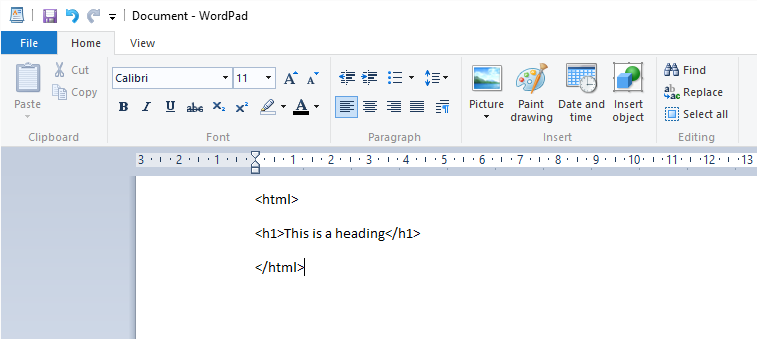
\includegraphics[width=.9\linewidth]{../../img/wordpadhtmldoc.png}
\subsection*{Then, save as a plain text file}
\label{sec:orgheadline16}
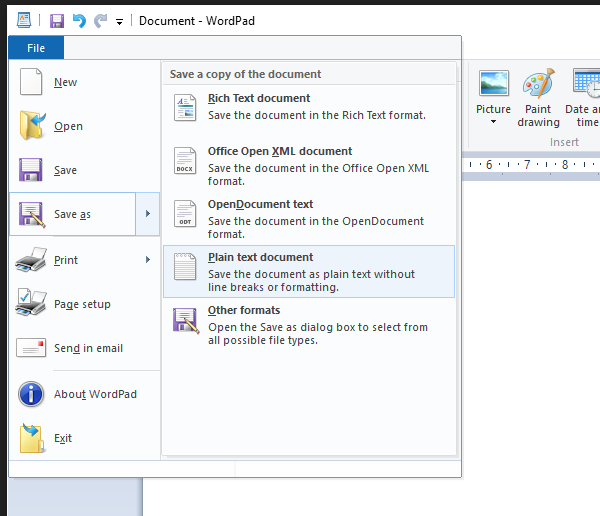
\includegraphics[width=.9\linewidth]{../../img/plaintextdoc.PNG}
\subsection*{When you get to the save dialogue}
\label{sec:orgheadline17}
\begin{itemize}
\item add '.html' to the end of the file name
\end{itemize}
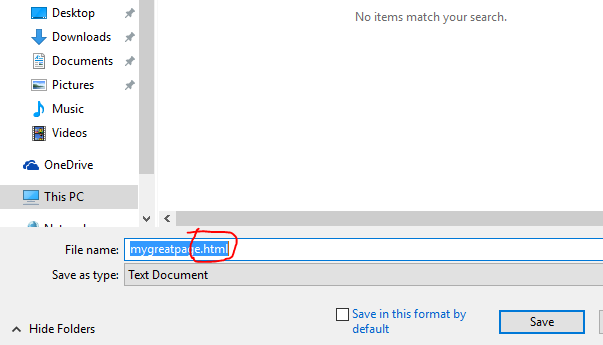
\includegraphics[width=.9\linewidth]{../../img/saveashtml.PNG}
\end{document}
